\section{Sistema de recomendação – Paradigma alternativo}

\subsection{Funcionamento do SCOAL}

Conforme explorado na seção anterior, o algoritmo \textit{k-NN} primeiramente
divide a matriz de dados em \textit{co-clusters} e, em seguida, realiza uma
predição baseada em um desses \textit{co-clusters} gerados. Tal algoritmo,
portanto, não leva em consideração os atributos dos filmes e dos usuários, isto
é, a predição é baseada exclusivamente nos \textit{ratings} dos usuários em uma
vizinhança. O algoritmo \textit{SCOAL}, por sua vez, utiliza ambas as
informações de vizinhança e atributos para predizer uma nota. A ideia do
\textit{SCOAL} é dividir toda a matriz em grupos, ou \textit{clusters}, de
maneira que cada um possa ser bem caracterizado por um único modelo preditivo. A
similaridade é dada, portanto, pela similiridade dos modelos preditivos e não
somente dos valores dos \textit{ratings}, como acontece no \textit{k-NN}. Além
disso, o \textit{SCOAL} realiza o agrupamento, ou \textit{co-clustering}, simultaneamente
com a obtenção dos respectivos modelos de classificação, a fim de melhorar a
designação dos dados aos \textit{clusters} e a precisão dos modelos.

\subsection{A base de dados \textit{MovieLens}}

Os dados utilizados nesta seção foram disponibilizados pelo grupo
\textit{GroupLens} no mês de Abril de 1998. São 100.000 \textit{ratings},
compreendidas no intervalo \([1,5]\), dadas por 943 usuários em 1682 filmes e
coletadas durante 7 meses, indo de 19 de setembro de 1997 até 22 de abril de
1998. É importante dizer que esses dados foram filtrados, de forma que usuários
com menos de 20 \textit{ratings} ou que não possuíssem informações
demográficas completas foram eliminados da base. Essas informações demográficas
são compostas por idade, sexo, ocupação e endereço \textit{zip}. Filmes, além
de informações sobre título, data de lançamento e \textit{url} do IMDb,
podem possuir diversos gêneros (ação, comédia, aventura etc). Destaca-se também
que a matriz é muito esparsa, isto é, muito de seus campos não estão
preenchidos.

\vspace{12pt}

Esses dados foram disponibilizados em alguns arquivos, cujos os principais são:

\begin{itemize}
  \item \texttt{u.data}: arquivo contendo as classificações dos usuários. Cada
  linha, além de possuir a respectiva \textit{rating}, associa um \textit{id} de
  usuário a um \textit{id} de filme. Adicionalmente, há um outro atribuot que
  descreve a data que a respectiva classificação foi dada.

  \item \texttt{u.item}: possui as informações apresentadas acima sobre os
  filmes.
  
  \item \texttt{u.user}: possui as informações apresentadas acima sobre os
  usuários.
  
\end{itemize}

\subsection{Execução do \textit{toolbox} fornecido}

O programa fornecido foi executado com 5 pastas para a \textit{k-fold
cross-validation}, 3 cortes nas linhas e 3 cortes nas colunas.
Foram gerados, portanto, 16 \textit{co-clusters}. Os coeficientes presentes na
tabela \ref{scoal:coef} foram obtidos para a iteração que apresentou menor MSE
(\textit{Mean Squared Error}). A imagem \ref{fig:scoal_result} representa o
valor deste indicador juntamente com alguns outros que avaliam o desempenho dos
preditores gerados, como. por exemplo, \textit{Precision} e \textit{Recall}. 

\FloatBarrier
	
	\begin{figure}[h]
    \centering
    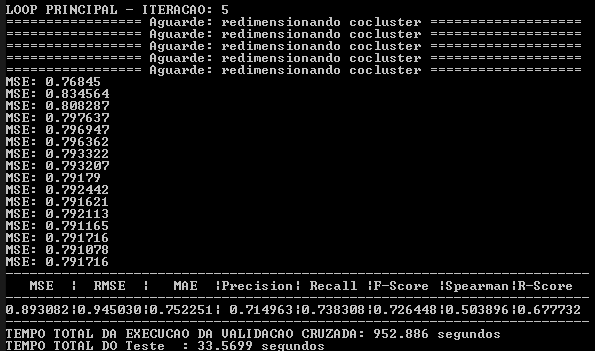
\includegraphics[scale=0.65]{scoal/execucaoScoal}
    \caption{\label{fig:scoal_result}Resultados para a 5ª iteração do
    algoritmo.}
	\end{figure}  
	
\FloatBarrier

\FloatBarrier
{\footnotesize
\begin{longtable}[h]{| c | p{0.9\textwidth} |} 

	\caption{\label{scoal:coef} Modelos preditivos para cada \textit{co-cluster}
	na iteração 5.}	\\
					
	\hline
	\textbf{Modelo} & \textbf{Coeficientes} \\ \hhline{|=|=|}
	1 & 0.145453; -0.305456; 0.041422; 0.118563; -0.100787; 0.100787; -0.361339;
	 -0.031360; -0.145453; 0.052350; 0.021124; 0.011262; 0.010038;
	-0.538674; -0.047585; -0.572105; -0.092489; -0.080133; -0.055039; -0.489122; 0.022816;
	-0.356975; -0.083862; 0.036848; 0.130115; -0.112789; -0.080782; 0.148531;
	-0.145453; 0.017635; 0.019313; -0.042312; 0.032170; 0.011268; -0.01965;
	0.037008; 0.027218; -0.003466; -0.055387; 0.006280; -0.039053; 0.006584;
	0.015461; -0.006752; -0.002389; 0.017252; -0.018370; -0.077912; 1.871064;
	-0.000088; \\ \hline
	2 & 0.158438; 0.098412; -0.084444; -0.172333; 0.098928; -0.098928; 0.114960;
	-0.237276; -0.033229; -0.216696; -0.133264; 0.131348; -0.468453; -0.232276;
	0.136819; -0.104005; -0.296712; -0.018775; 0.036848; -0.123124; -0.286383;
	-0.046800; -0.222357; -0.032034; -0.350149; -0.169591; -0.458762;
	-0.010351; -0.158438; 0.024304; 0.017394; 0.003218; -0.040178; -0.006777;
	-0.008178; 0.165993; -0.026013; -0.024336; 0.019608; -0.019747; 0.082755;
	-0.050241; 0.009563; 0.023744; 0.006748; -0.006169; -0.021861; -0.010928;
	1.978979; -0.338162; \\ \hline
	3 & 0.154957; 0.140657; -0.130708; -0.164910; -0.001337; 0.001337;
	-0.107116; -0.486860; -0.235860; -0.210768; -0.361360; -0.228055; -0.126928;
	0.125811; -0.027875; -0.081434; -0.067236; -0.402994; -0.304448; 0.082657;
	0.055919; -0.188501; 0.159001; -0.225646; -0.062895; -0.278069; 0.027141;
	0.036943; -0.154957; 0.013116; 0.003827; -0.004108; -0.055794; -0.003045;
	-0.009006; -0.125374; -0.004883; 0.011032; -0.000223; 0.036841; 0.004948;
	0.045497; -0.000247; -0.016238; 0.028038; 0.004095; 0.044256; 0.004544;
	1.914104; -0.363268 ; \\ \hline 
	4 & 0.160529; 0.007257; -0.117741; -0.050074; -0.018830; 0.018830; -0.112880;
	-0.150154; 0.128904; -0.145439; -0.064703; -0.187139; -0.365357; -0.049431;
	-0.576610; -0.005741; -0.242354; -0.274566; 0.188305; -0.146628; -0.154143;
	-0.511182; 0.103514; -0.154050; -0.053636; 0.063296; -0.346568; -0.294042;
	-0.160529; -0.062514; -0.033490; 0.011760; -0.009649; 0.028094; 0.037871;
	0.019659; 0.037787; 0.081594; 0.027281; 0.011614; 0.008447; -0.025850;
	-0.015608; -0.000924; -0.032736; -0.015211; -0.009934; 0.041682; 2.259185;
	0.176226; \\ \hline 
	5 & 0.153238; -0.289953; 0.056217; 0.080444; -0.176394;
	0.176394; -0.272798; -0.345049; -0.153238; 0.060464; 0.061706; -0.235400;
	0.112666; -0.929689; -0.127659; -0.791338; 0.004033; -0.168081; -0.072029;
	-0.360590; 0.142148; -0.094107; -0.204140; 0.150260; 0.112863; -0.007595;
	0.204809; 0.205846; -0.153238; 0.012859; -0.017582; -0.033241; 0.029942;
	-0.022328; -0.018988; -0.081810; -0.009810; 0.120705; -0.081946; 0.167287;
	-0.059177; 0.000068; 0.000693; 0.030118; 0.025867; -0.000215; -0.026430;
	0.026859; 2.078046; 0.163905; \\ \hline 
	6 & 0.209385; -0.615300; 0.275593;
	0.130311; -0.269474; 0.269474; -0.166631; -0.324050; -0.209385; 0.314726;
	-0.031355; -0.600633; 0.233076; 0.036878; -0.645836; -0.776475; -0.369757;
	0.416463; -0.554884; -0.567367; 0.048666; 0.463706; -0.531050; -0.209385;
	0.149720; -0.001071; -0.654194; 0.093764; -0.209385; 0.130455; 0.056835;
	-0.222108; 0.086176; 0.011397; 0.352807; 0.090408; -0.099081; -0.172382;
	-0.283249; 0.001985; 0.146003; 0.214892; -0.122668; 0.044627; -0.096482;
	0.454269; 0.216841; 0.011747; 1.363391; 0.286857; \\ \hline 
	7 & 0.074156;
	-0.276172; 0.156241; 0.045794; -0.153727; 0.153727; -0.169476; 0.292783;
	-0.074156; 0.281942; 0.060345; -0.116324; -0.031924; -0.460518; -0.364804;
	-0.150334; 0.081755; 0.013356; 0.034094; -0.531589; 0.069247; 0.279620;
	-0.135149; -0.477126; 0.135330; -0.167795; 0.021751; 0.169321; 0.059546;
	0.140365; 0.112379; -0.142606; 0.132601; 0.024045; 0.082573; -0.056270;
	0.040479; -0.828516; -0.107644; 0.012118; -0.106625; -0.063357; 0.015247;
	0.098645; 0.052261; 0.196016; -0.317204; -1.302668; 1.844769; 0.773247;\\ \hline
	8 & 0.159554; 0.130232; -0.149348; -0.140438; 0.071082; -0.071082; 0.079011;
	0.161992; -0.059673; -0.132908; -0.259776; 0.116072; -0.766087; -0.263210;
	-0.119554; -0.139388; -0.213015; 0.004084; 0.484236; -0.130024; -0.291548;
	-0.072007; -0.454042; -0.178572; -0.410951; -0.170437; -0.215582; -0.039038;
	-0.159554; 0.063759; -0.014169; 0.026256; -0.027020; -0.000913; 0.025837;
	0.059471; -0.062676; -0.091991; -0.109653; 0.076020; 0.054455; -0.056571;
	-0.021649; -0.070765; -0.019649; 0.012628; -0.020391; 0.168960; 1.712372;
	-0.158062;\\ \hline 
	9 & 0.165744; 0.072184; -0.141980; -0.095928; -0.082982;
	0.082982; -0.186644; -0.866382; -0.170484; -0.250890; -0.399213; 0.008862;
	-0.057555; 0.085714; -0.161120; 0.336326; -0.139211; -0.276578; -0.238796;
	-0.024920; -0.014957; 0.023362; -0.160613; -0.180117; -0.088914; -0.298469;
	-0.090202; 0.055767; -0.165744; -0.038946; -0.007102; 0.101837; -0.014165;
	-0.059708; 0.001603; 0.051558; -0.014857; -0.087410; 0.053863; -0.008801;
	-0.152968; 0.007850; 0.015132; 0.039744; 0.002453; 0.034771; 0.055539;
	-0.118275; 1.708164; -0.080727; \\ \hline 
	10 & 0.117609; 0.121627; -0.282165;
	0.042916; -0.058406; 0.058406; 0.107498; -0.117609; -0.019190; -0.405692;
	-0.273367; -0.255412; -0.549664; -0.314560; -0.176684; -0.181694; -0.070138;
	0.562161; 0.836102; -0.059110; 0.195050; 0.036555; -0.622938; 0.178962;
	-0.181715; -0.150814; -0.772024; -0.172533; -0.117609; -0.053115; 0.153536;
	0.002256; -0.200794; -0.038823; -0.042921; -0.217099; -0.032497; 0.067446;
	-0.117609; 0.036354; -0.125077; 0.375880; -0.025930; -0.304797; 0.088381;
	-0.225396; -0.092929; -0.273183; 0.864530; -0.211613;\\ \hline 
	11 & 0.075682;
	0.014163; -0.047494; -0.042352; -0.113082; 0.113082; -0.050384; 0.136660;
	0.092318; 0.078522; -0.203886; 0.599453; -0.554428; 0.183884; -0.075682;
	-0.075682; -0.049259; -0.770246; 0.006306; -0.288197; -0.184931; -0.765363;
	0.041453; 0.315831; 0.098852; 0.079702; -0.052735; 0.480192; -0.075682;
	-0.180874; -0.148958; 0.356630; -0.223928; -0.082032; -0.277486; -0.068537;
	0.094255; 0.013841; -0.075682; 0.137614; 0.009946; -0.565146; -0.112763;
	-0.057013; 0.234001; 0.189301; -0.070850; -0.739999; 2.326597; 0.268200;  \\
	\hline 
	12 & 0.191561; -0.193858; 0.029130; -0.026836; 0.042587; -0.042587;
	-0.089181; 0.203084; -0.089162; -0.331050; -0.134555; -0.033791; -1.134447;
	-0.247984; -0.280799; -0.576608; -0.018402; 0.212571; 0.702313; -0.195558;
	-0.476448; 0.163142; -0.087483; -0.088211; -0.307796; -0.229101; -0.599600;
	0.064498; 0.093746; -0.011906; -0.013979; 0.111372; 0.037223; 0.008758;
	-0.065282; -0.143293; 0.016528; 0.150781; -0.044906; 0.039258; -0.196244;
	-0.079988; -0.003830; 0.047696; -0.041619; 0.218680; 0.006091; 0.417986;
	1.150833; -0.683341; \\ \hline
	13 & 0.148209; -0.059039; -0.083705; -0.005491; 0.010328; -0.010328; -0.230760;
	-0.189309; -0.538609; -0.103990; 0.219079; -0.530764; 0.356418; -0.322340;
	-0.148209; -0.368023; 0.144423; -0.091621; -0.148209; 0.105816; -0.121599;
	-0.270846; -0.081490; -0.203113; -0.148463; 0.199290; -0.343332; -0.031252;
	-0.148209; 0.040285; -0.041633; -0.027047; -0.062109; -0.001586; -0.117222;
	0.468140; 0.015223; -0.018937; 0.003423; 0.318983; -0.146294; -0.111940;
	0.022961; -0.028951; 0.099396; 0.064670; 0.151182; -0.592075; 2.222140;
	-0.427067;  \\ \hline
	14 & 0.175461; 0.036977; -0.155914; -0.056518; -0.062314; 0.062314; -0.268933;
	0.518875; -0.288730; -0.108100; -0.236450; -0.343871; 0.376072; -0.026862;
	-0.173402; 0.024717; -0.137289; -0.561450; -0.004052; -0.388198; -0.188005;
	0.063221; -0.817763; 0.035023; -0.129884; -0.356983; -0.320587; -0.060569;
	-0.440755; 0.005263; 0.151253; 0.187391; -0.000756; -0.047214; -0.044171;
	0.091214; -0.025574; -0.001232; 0.264114; -0.041650; 0.074576; 0.014387;
	-0.036335; 0.107233; -0.067227; -0.029637; -0.045870; -0.114915; 2.653960;
	0.109496; \\ \hline
	15 & 0.183501; -0.230915; 0.040334; 0.007055; -0.124662; 0.124662; -0.219916;
	-0.402084; 0.738653; -0.155448; -0.319779; -0.025436; -0.121768; -1.444828;
	-0.108418; -1.038054; -0.111564; 0.172685; -0.059428; -0.219212; -0.050784;
	-0.056240; -0.045836; -0.002217; 0.205654; 0.066217; -0.287053; -0.174689;
	0.045627; -0.023441; -0.003491; 0.187322; -0.103295; 0.034463; 0.040738;
	0.033431; 0.042559; 0.197273; -0.092128; 0.002823; -0.188358; 0.063411;
	-0.013565; 0.022282; -0.067198; -0.005062; 0.033840; 0.002839; 1.283242;
	0.430237;  \\ \hline
	16 & 0.129548; -0.192931; -0.011378; 0.074778; 0.100693; -0.100693; -0.372648;
	0.139234; 0.183694; -0.123371; 0.039792; 0.270973; 0.124380; -0.287096;
	-0.129548; -0.449262; 0.088444; -0.109449; -0.125029; -0.038168; -0.250164;
	-0.562955; 0.147216; -0.321983; -0.172657; -0.137911; -0.374117; -0.154699;
	-0.076793; -0.066423; -0.147318; 0.158223; -0.055649; 0.025543; 0.178691;
	0.034346; 0.057687; 0.030371; -0.253588; -0.203573; 0.024121; 0.041857;
	0.028999; -0.006382; -0.032658; 0.010550; 0.014744; -0.182972; 1.916620;
	-0.008113; \\ \hline
			    
	\end{longtable} }

\FloatBarrier


O programa foi utilizado para prever resultados de um usuário
escolhido aleatoriamente, cujo \textit{id} vale 102. Os resultados estão
presentes na tabela \ref{tab:scoal_102}. Verifica-se que os piores erros são
realizados para notas baixas dadas pelo usuário, isto é, para os filmes que
usuário avaliou como 1, os modelos produziram notas superiores a 3. Este fato
decorre da característica esparsa da matriz: o algoritmo não possui
\textit{ratings} suficientes para avaliar com qualidade todas as notas.

\FloatBarrier
	
	\begin{table}[h]
	    \centering
		\caption{\label{tab:scoal_102} Comparação entre valores dados e preditos para
		o usuário 102.}
		\begin{tabular}{| c | c | c | }
			\hline
			\textbf{Filme} & \textbf{Valor Previsto} & \textbf{Valor Dado} \\ \hline
			809 & 3.44625 & 3 \\ \hline
			672 & 3.66343 & 1 \\ \hline
			986 & 3.18711 & 1 \\ \hline
			612 & 4.18292 & 4\\ \hline
			515 & 4.79791 & 1 \\ \hline
			67  & 3.48557 & 1 \\ \hline
		\end{tabular}	    
    \end{table}
    
    \FloatBarrier

\subsection {As medidas de qualidade de predição}

Uma parte importante na tarefa de predição é a capacidade de avaliar os
resultados obtidos. Assim como fizemos durante todo o curso, utiliza-se parte do
conjunto de dados para validação e testes para medir o quão boa foi uma
recomendação gerada pelo sistema. Define-se, portanto, algumas medidas que
relacionam os resultados dos modelos preditivos aplicados nos dados de testes
com os respectivos valores atribuídos pelos usuários e, dessa forma, é possível
medir aspectos pontuais dos modelos calculados.

\vspace{12pt}

Destacam-se três medidores:

\begin{itemize}
  \item \textbf{Mean Squared Error - MSE}: é a média da soma das diferenças
  entre os valores preditos e os reais ao quadrado. Para a figura
  \ref{fig:scoal_result},  verifica-se que este atributo é calculado para cada
  \textit{co-cluster} durante o processo de treinamento/validação dos modelos.
  Destaca-se que, neste caso, foi utilizada a técnica de \textit{k-fold
  crossvalidation}, sendo que todos os dados são utilizados pelo menos uma vez
  como dados de validação. Foi observado que estes valores ficaram próximos de
  0.800. Calcula-se também, ao fim, conforme indicado na parte inferior da
  imagem \ref{fig:scoal_result}, o \textit{MSE} obtido em relação ao dados de teste.
  Para a melhor iteração, a 5ª, obtém-se \(MSE = 0.8931\).
 
  \item \textbf{Precision}: em poucas palavras, este medidor é a fração dos
  resultados encontrados que são relevantes, isto é, são valores acertados pelo
  sistema. Neste caso, este parâmetro é definido por
 
  \begin{equation}
  P_{precision} = \frac{V_P}{V_P + F_P}
  \end{equation}
 
 
  em que \(V_P\), ou \textit{verdadeiros positivos}, é o total de avaliações
  superiores ou iguais a 4 feitas pelo sistema para os dados de teste e
  \(F_P\), ou \textit{falsos positivos}, é o total destas avaliações que o
  sistema calculou erroneamente, isto é, um valor predito deveria ser inferior
  a 4 conforme o respectivo  valor real. O valor obtido para este medidor na 5ª
  iteração foi 0.7150, o que indica que o sistema tem aproximadamente 70\% de
  precisão em suas predições.
 
  \item \textbf{Recall}: este parâmetro mede a fração de valores relevantes
  encontrados pelo sistema. Definido por:
 
  \begin{equation}
  R_{recall} = \frac{V_P}{V_P + F_N}  = \frac{\%_{V_P}}{T_{predicoes}}
  \end{equation}
 
  em que \(F_N\), ou \textit{falso negativo}, é o número de notas que foram
  preditas erroneamente sendo menor que 4,  \(V_P\) é o total de boas predições
  feitas pelo sistema e que são superiores ou iguais a 4 e \(T_{predicoes}\) é
  total de avaliações superiores ou iguais a 4 realizadas.  O valor obtido para
  este medidor na 5ª iteração foi 0.7383, indicando que um grau de
  acertabilidade adequado.
 
\end{itemize}